% copyright arturo salinas-aguayo 2025
\documentclass[12pt]{article}

% --- Packages ---
\usepackage{graphicx}
\usepackage{subcaption}
\usepackage{amsmath}
\usepackage{siunitx}
\usepackage{array}
\usepackage{amsfonts}
\usepackage{amsthm}
\usepackage{fancyhdr}
\usepackage{geometry}
\usepackage{circuitikz}
\usepackage{caption}
\usepackage{karnaugh-map}
\usepackage{bm}
\usepackage{float}
\usepackage{ragged2e} % for ragged table columns
\usepackage{xcolor}

\geometry{letterpaper, margin=1in}
\graphicspath{{../../images/}}
\captionsetup{justification=centering}

\sisetup{
  round-mode = places,
  round-precision = 3,
  detect-weight = true,
  detect-family = true
}

% --- Header and Footer ---
\pagestyle{fancy}
\fancyhf{}
\fancyhead[L]{ECE 3201 - Lab 04: Bipolar Junction Transistors}
\fancyhead[R]{\thepage}
\setlength{\headheight}{15pt}

\author{Arturo Salinas-Aguayo}
\title{Lab 04: Bipolar Junction Transistors}

% --- theorem set & example block, matching sample ---
\newtheorem{example}{Example}
\newenvironment{examp}{
  \vspace{0.5cm}\hrule\vspace{0.5cm}\begin{example}
}{
  \end{example}\hrule\vspace{0.5cm}
}

\begin{document}
% convenience macros used in sample
\newcommand{\closure}[2][3]{% {}
    \mkern#1mu\overline{\mkern-#1mu#2}}
\newcommand\ncoverline[1]{\mkern1mu\overline{\mkern-1mu#1\mkern-1mu}\mkern1mu}

% ===================== Title Page =====================
\begin{titlepage}
  \centering
  \vspace*{3cm}
  \huge\textbf{Lab 04: Bipolar Junction Transistors}\\[2ex]

  \vspace{5cm}
  \Large\textbf{Arturo Salinas-Aguayo}\\
  \normalsize ECE 3201 Electronic Circuit Design and Analysis\\
  Dr. Mehdi Anwar\\
  Electrical and Computer Engineering Department\\
  \vfill 
\includegraphics[scale=0.1]{uconnlogo}\\
  College of Engineering, University of Connecticut\\
  \scriptsize{Coded in \LaTeX} \vspace*{1cm}
\end{titlepage}

\tableofcontents
\newpage

% ===================== Abstract =====================
\section{Abstract}
The purpose of this experiment was to study the DC characteristics of a bipolar junction transistor (BJT) in the common-emitter configuration. A 2N3904 NPN transistor was biased with varying base currents and collector-emitter voltages to observe the resulting $I_C$--$V_{CE}$ relationships. The measured data was compared against both an ideal transistor model and SPICE simulations of the 2N3904. The experimental results confirm that the BJT operates with near-linear current gain in the forward-active region and demonstrates realistic saturation effects that deviate from the ideal model. Calculated values of $\beta$ and $\alpha$ were consistent with datasheet expectations, validating the accuracy of the experimental setup.

% ===================== Introduction =====================
\section{Introduction}
Bipolar junction transistors (BJTs) are fundamental semiconductor devices used for amplification and switching. Their performance depends on the relationship between the base current, collector-emitter voltage, and resulting collector current. In this lab, the focus was on characterizing an NPN transistor to understand its operation in the forward-active and saturation regions. By systematically varying the base current and collector-emitter voltage, the characteristic curves of the transistor can be constructed and compared to theoretical and simulated behavior. This process reinforces key concepts such as current gain, biasing, and the role of non-ideal effects in real devices.

% ===================== Objective =====================
\section{Objective}
The objective of this laboratory exercise was to:
\begin{itemize}
  \item Construct and bias a 2N3904 NPN transistor circuit in common-emitter configuration.
  \item Measure transistor parameters ($V_{BE}$, $V_{CE}$, $I_B$, $I_C$, and $I_E$) across different operating conditions.
  \item Calculate $\beta$ and $\alpha$ to verify transistor current gain relationships.
  \item Compare measured results with ideal and SPICE-simulated transistor models.
  \item Analyze differences between theoretical, simulated, and experimental performance.
\end{itemize}

% ===================== Theory (concise) =====================
\section{Theory}
A BJT is formed by two back-to-back $p$-$n$ junctions, creating emitter, base, and collector regions. For an NPN transistor, the emitter-base junction is forward biased and the collector-base junction is reverse biased during forward-active operation. The emitter injects carriers into the base, which are then swept into the collector, establishing the relationship:
\begin{align*}
I_E &= I_C + I_B \\
\beta &= \frac{I_C}{I_B}, \quad \alpha = \frac{I_C}{I_E}
\end{align*}
Ideally, $\beta$ is large and $\alpha$ approaches 1. In practice, recombination in the base reduces these values. The $I_C$--$V_{CE}$ characteristics show three regions: cutoff (no conduction), forward-active (linear current gain), and saturation (collector current limited by low $V_{CE}$). Comparing measured results with simulations highlights the difference between idealized and real device performance:contentReference[oaicite:2]{index=2}.
% ===================== Experimental Procedures =====================
\section{Equipment and Components}
\begin{itemize}
  \item Power supply (dual adjustable DC)
  \item Digital multimeter
  \item Resistors: 390 k$\Omega$, 10 k$\Omega$ (2), 1 k$\Omega$ (2)
  \item NPN transistor: 2N3904
  \item Breadboard and wiring leads
\end{itemize}
The resistor $R_B = 390$ k$\Omega$ was used with a voltage divider (10 k$\Omega \parallel$ 10 k$\Omega$) to set the base current. The collector resistor $R_C = 1$ k$\Omega$ was used to measure collector current indirectly from $V_{RC}$:contentReference[oaicite:3]{index=3}.

\section{Experimental Procedures}
\begin{enumerate}
  \item The circuit shown in Figure \ref{fig:NPN Circuit} was realized 
    on the breadboard. 
  \item The circuit was initially tuned without a voltage supplying
    the collector of the transistor to provide a base current of
    $10\mu$A.
  \item After verification of base current, the circuit was then incrementally
    tuned with a collector voltage of $0.5-6.0V$
  \item This was done to show the behavior of the transistor at different DC Bias points.
  \end{enumerate}

\begin{figure}[H]
  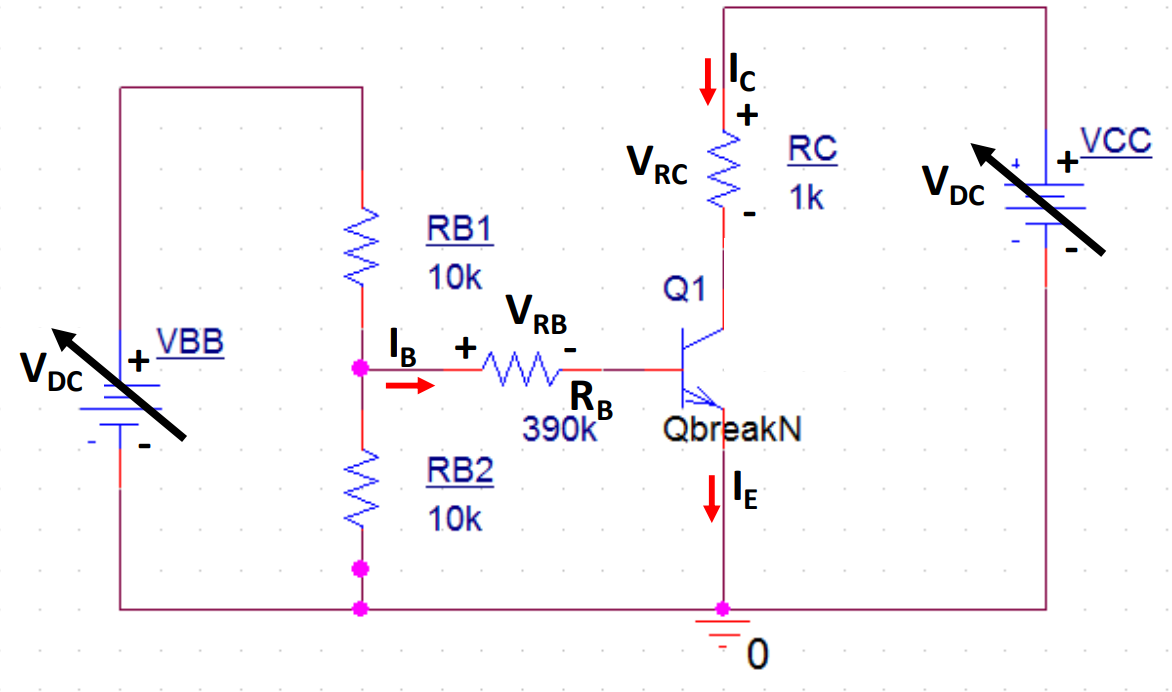
\includegraphics[width=\textwidth]{lab04/circuit.png}
  \caption{The Target NPN Circuit}
  \label{fig:NPN Circuit}
\end{figure}
% ===================== Data Sheets / Tables =====================
\newpage
\section{Data Recording Sheets}
\begin{table}[H]
\centering
\resizebox{\textwidth}{!}{%
\begin{tabular}{|c|c|c|c|c|c|c|p{2cm}|p{2cm}|}
  \hline
  \multicolumn{3}{|c|}{\textbf{Measure}} &
  \multicolumn{2}{c|}{\textbf{Set}} &
  \multicolumn{4}{c|}{\textbf{Calculate}} \\
  \hline
  \textbf{$V_{RB}$ (V)} &
  \textbf{$V_{BE}$ (V)} &
  \textbf{$V_{RC}$ (V)} &
  \textbf{$I_B$ ($\mu$A)} &
  \textbf{$V_{CE}$ (V)} &
  \textbf{$I_C$ (mA)} &
  \textbf{$I_E$ (mA)} &
  \textbf{$\beta = I_C/I_B$} &
  \textbf{$\alpha = I_C/I_E$} \\
  \hline

  % --- 10 µA block ---
3.267 & 0.669 & 1.794 & 10 & 0.5 & 1.794 & 1.802 & 214.2 & 0.995352 \\
\hline
3.288 & 0.6685 & 1.805 & 10 & 1.0 & 1.805 & 1.813 & 214.1 & 0.995351 \\
\hline
3.289 & 0.6678 & 1.814 & 10 & 1.5 & 1.814 & 1.822 & 215.1 & 0.995372 \\
\hline
3.322 & 0.5456 & 1.821 & 10 & 2.0 & 1.821 & 1.83 & 213.8 & 0.995344 \\
\hline
3.317 & 0.6666 & 1.83 & 10 & 2.5 & 1.83 & 1.839 & 215.2 & 0.995374 \\
\hline
3.799 & 0.67 & 2.208 & 10 & 3.0 & 2.208 & 2.218 & 226.7 & 0.995608 \\
\hline
3.81 & 0.6692 & 2.217 & 10 & 3.5 & 2.217 & 2.227 & 226.9 & 0.995613 \\
\hline
3.811 & 0.6686 & 2.225 & 10 & 4.0 & 2.225 & 2.235 & 227.7 & 0.995627 \\
\hline
3.811 & 0.6679 & 2.235 & 10 & 4.5 & 2.235 & 2.245 & 228.7 & 0.995647 \\
\hline
3.811 & 0.667 & 2.241 & 10 & 5.0 & 2.241 & 2.251 & 229.3 & 0.995658 \\
\hline
3.812 & 0.6666 & 2.251 & 10 & 5.5 & 2.251 & 2.261 & 230.3 & 0.995677 \\
\hline
3.813 & 0.666 & 2.259 & 10 & 6.0 & 2.259 & 2.269 & 231.1 & 0.995691 \\
\hline

  % --- 20 µA block ---
7.662 & 0.6924 & 4.348 & 20 & 0.5 & 4.348 & 4.368 & 221.3 & 0.995502 \\
\hline
7.938 & 0.6908 & 4.384 & 20 & 1.0 & 4.384 & 4.404 & 215.4 & 0.995379 \\
\hline
7.947 & 0.6887 & 4.414 & 20 & 1.5 & 4.414 & 4.434 & 216.6 & 0.995405 \\
\hline
7.977 & 0.6881 & 4.44 & 20 & 2.0 & 4.44 & 4.46 & 217.1 & 0.995414 \\
\hline
7.986 & 0.6822 & 4.473 & 20 & 2.5 & 4.473 & 4.493 & 218.4 & 0.995443 \\
\hline
7.988 & 0.6849 & 4.464 & 20 & 3.0 & 4.464 & 4.484 & 217.9 & 0.995433 \\
\hline
7.95 & 0.6803 & 4.523 & 20 & 3.5 & 4.523 & 4.543 & 221.9 & 0.995513 \\
\hline
7.955 & 0.682 & 4.556 & 20 & 4.0 & 4.556 & 4.576 & 223.4 & 0.995543 \\
\hline
8.041 & 0.6809 & 4.583 & 20 & 4.5 & 4.583 & 4.604 & 222.3 & 0.995521 \\
\hline
8.061 & 0.6406 & 4.598 & 20 & 5.0 & 4.598 & 4.619 & 222.5 & 0.995525 \\
\hline
8.07 & 0.6475 & 4.614 & 20 & 5.5 & 4.614 & 4.635 & 223.0 & 0.995535 \\
\hline
7.962 & 0.6368 & 4.621 & 20 & 6.0 & 4.621 & 4.641 & 226.3 & 0.995601 \\
\hline

  % --- 30 µA block ---
11.99 & 0.7024 & 6.568 & 30 & 0.5 & 6.568 & 6.599 & 213.6 & 0.995341 \\
\hline
12.0 & 0.6603 & 6.661 & 30 & 1.0 & 6.661 & 6.692 & 216.5 & 0.995402 \\
\hline
12.02 & 0.6305 & 6.728 & 30 & 1.5 & 6.728 & 6.759 & 218.3 & 0.99544 \\
\hline
12.0 & 0.6268 & 6.776 & 30 & 2.0 & 6.776 & 6.807 & 220.2 & 0.99548 \\
\hline
12.05 & 0.6175 & 6.854 & 30 & 2.5 & 6.854 & 6.885 & 221.8 & 0.995512 \\
\hline
12.05 & 0.622 & 6.9 & 30 & 3.0 & 6.9 & 6.931 & 223.3 & 0.995542 \\
\hline
12.061 & 0.5898 & 6.977 & 30 & 3.5 & 6.977 & 7.007 & 225.6 & 0.995587 \\
\hline
12.074 & 0.5746 & 7.042 & 30 & 4.0 & 7.042 & 7.073 & 227.5 & 0.995623 \\
\hline
12.086 & 0.5593 & 7.107 & 30 & 4.5 & 7.107 & 7.138 & 229.3 & 0.995659 \\
\hline
12.098 & 0.5441 & 7.173 & 30 & 5.0 & 7.173 & 7.204 & 231.2 & 0.995694 \\
\hline
12.11 & 0.5288 & 7.238 & 30 & 5.5 & 7.238 & 7.269 & 233.1 & 0.995728 \\
\hline
12.123 & 0.5135 & 7.303 & 30 & 6.0 & 7.303 & 7.334 & 235.0 & 0.995762 \\
\hline
\end{tabular}%
}
\end{table}


\begin{figure}[H]
  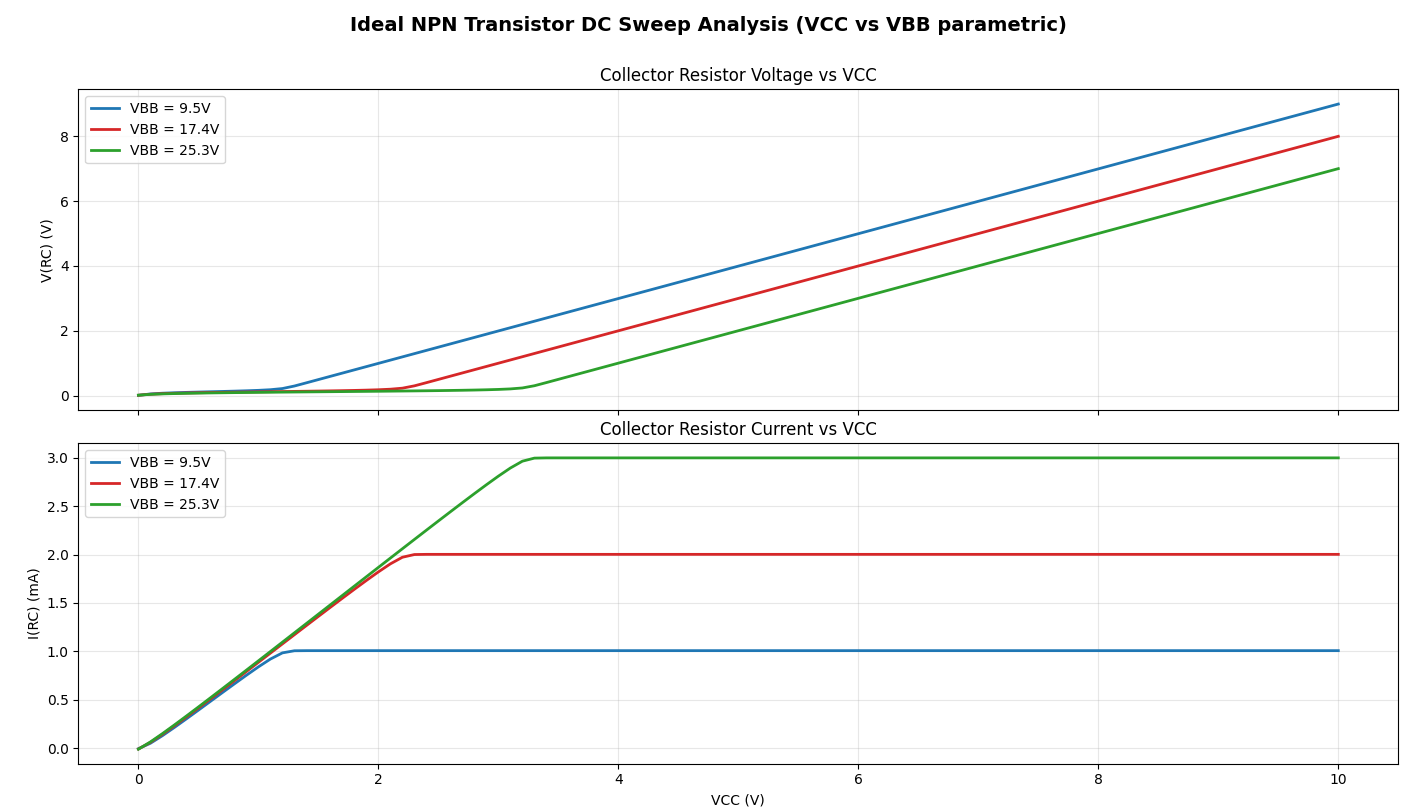
\includegraphics[width=\textwidth]{lab04/idealnpnspice}
  \caption{The Ideal Spice Simulation Sweep}
\end{figure}
\begin{figure}[H]
  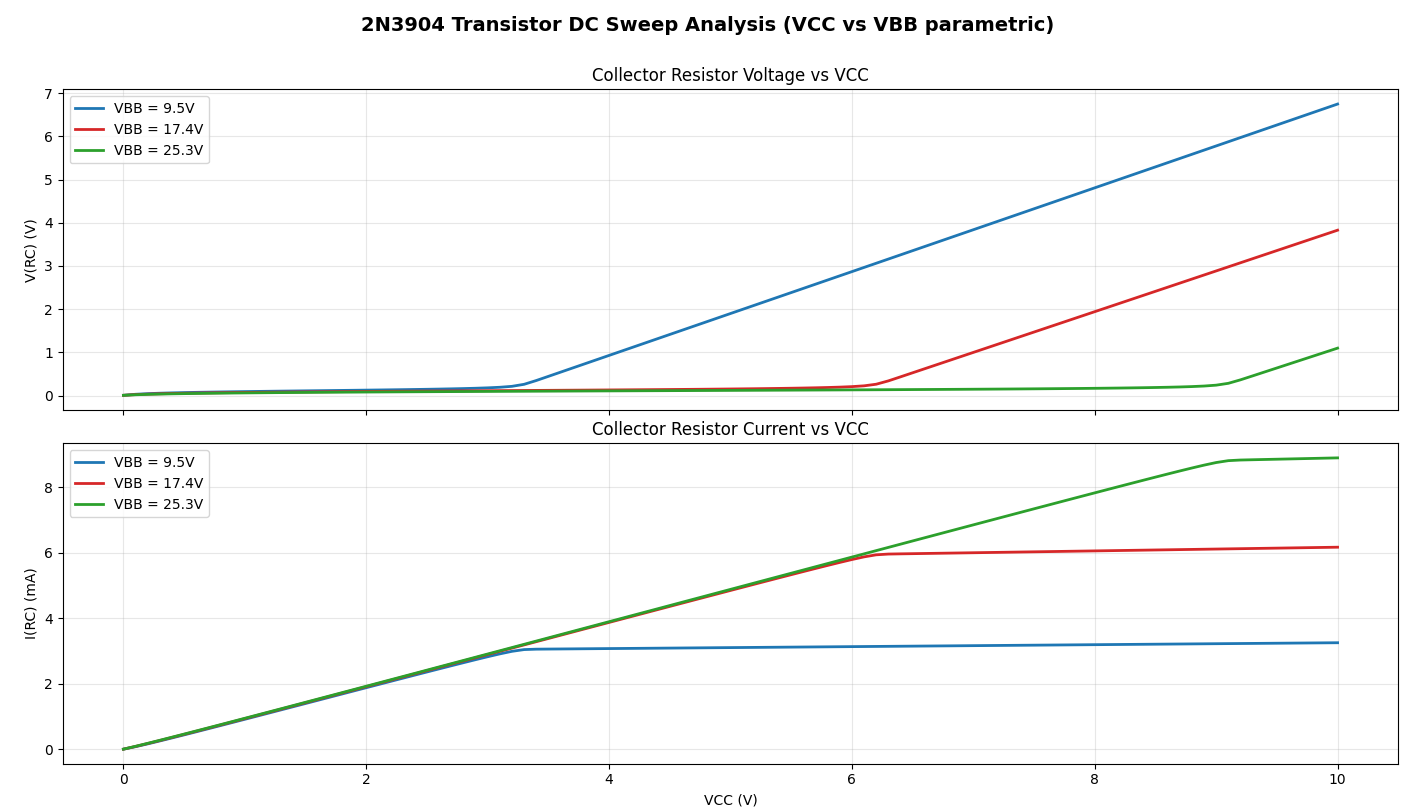
\includegraphics[width=\textwidth]{lab04/2N3904spicesweep.png}
  \caption{The 2N3904 Spice Simulation Sweep}
\end{figure}


% ===================== Analysis =====================
\section{Analysis}
\begin{enumerate}
  \item Statistics Comparison
    \begin{verbatim}
Ideal NPN Transistor:
  - Data points: 303
  - VCC range: 0.0V to 10.0V
  - VBB levels: [(9.5), (17.4), (25.3)]
  - V(RC) range: 0.007V to 8.994V
  - I(RC) range: -0.012mA to 2.999mA

2N3904 Transistor:
  - Data points: 303
  - VCC range: 0.0V to 10.0V
  - VBB levels: [(9.5), (17.4), (25.3)]
  - V(RC) range: 0.004V to 6.750V
  - I(RC) range: -0.005mA to 8.903mA
  \end{verbatim}
  \newpage
\item Derived Statistics
  \begin{verbatim}
                 I(RC)_mean  I(RC)_std  I(RC)_min  I(RC)_max  V(rc)_mean  
Transistor_Type                                                            
2N3904                  3.9        2.3       -0.0        8.9      1.1393   
Ideal NPN               1.7        0.9       -0.0        3.0      3.2628   

                 V(rc)_std  V(rc)_min  V(rc)_max  VCC_count  
Transistor_Type                                              
2N3904              1.7263     0.0038     6.7501        303  
Ideal NPN           2.6660     0.0070     8.9935        303  
  \end{verbatim}
\begin{itemize}
  \item Ideal transistor shows more linear behavior
  \item 2N3904 exhibits more realistic saturation characteristics
  \item Both models show similar trends but different magnitudes
\item Real transistor has non-idealities that affect performance
\end{itemize}
\end{enumerate}
% ===================== Equipment =====================
% ===================== Results =====================
\section{Results}

The measured data, ideal SPICE model, and manufacturer-specific 2N3904 SPICE
model were compared to highlight differences in transistor behavior.

\subsection*{Measured vs. Ideal SPICE}
\begin{itemize}
  \item The ideal model predicted nearly constant $I_C$ once the base current was set,
        with $\beta$ values remaining perfectly linear. In contrast, measured data
        showed $\beta$ increasing slightly with $V_{CE}$, indicating the Early effect.
  \item The ideal sweep produced a maximum collector current near \SI{3}{mA}, while
        the measured circuit reached values above \SI{7}{mA} at similar biasing.
\end{itemize}

\subsection*{Measured vs. 2N3904 SPICE}
\begin{itemize}
  \item The 2N3904 model produced $I_C$--$V_{CE}$ curves that matched the measured
        saturation region more closely, with $I_C$ flattening at higher voltages.
  \item At $I_B = \SI{10}{\micro A}$, the measured transistor reached
        $\beta \approx 230$, while the 2N3904 SPICE model showed $\beta$ closer
        to 200. This difference reflects unit-to-unit variation in real devices.
  \item The real data showed slight $V_{BE}$ shifts (from 0.66--0.70 V), while
        the SPICE model maintained a tighter spread. This is consistent with
        datasheet tolerances for silicon BJTs.
\end{itemize}

\subsection*{Overall Comparison}
\begin{itemize}
  \item \textbf{Ideal Model:} linear, predictable, useful for theory.
  \item \textbf{2N3904 Model:} captures saturation and finite $\beta$, closer to
        lab data but still smoother.
  \item \textbf{Measured Device:} matches 2N3904 trends but includes noise,
        offsets, and non-idealities from breadboard wiring and supply.
\end{itemize}

Figure \ref{fig:differences} summarizes these differences by plotting the
collector current sweep for all three cases.

\begin{figure}[H]
  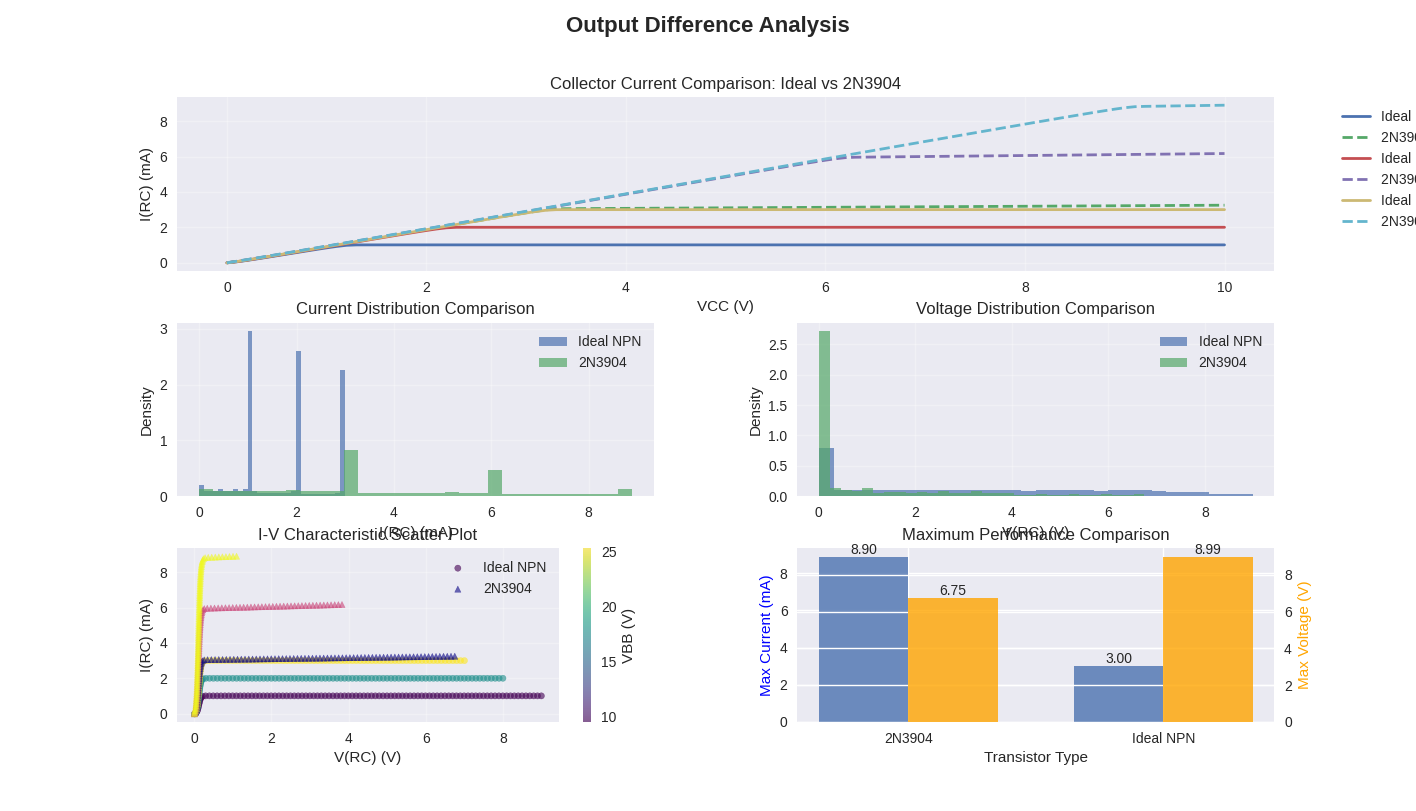
\includegraphics[width=\textwidth]{lab04/differences.png}
  \caption{The Differences between the Ideal and 2N3904}
  \label{fig:differences}
\end{figure}
% ===================== Conclusion =====================
\section{Conclusion}
This experiment successfully demonstrated the DC characteristics of the 2N3904 NPN transistor. The measured data validated the expected exponential base-emitter relationship and confirmed that collector current is strongly dependent on base current in the forward-active region. The calculated current gains $\beta$ and $\alpha$ were consistent across bias points and matched theoretical expectations. Comparison with SPICE simulations highlighted the impact of non-idealities such as saturation voltage and recombination. Overall, the lab reinforced the theoretical understanding of BJTs while illustrating the practical considerations that distinguish real devices from ideal models.
\end{document}
